\section{La tournée du facteur}

Un facteur doit distribuer du courrier dans $n$ maisons différentes. Les coordonnées de ces maisons (qui sont supposées se trouver dans un village parfaitement plat) sont repérées par deux tableaux de flottants \texttt{x} et \texttt{y} de taille $n$.
\medskip

La $i$-ième maison est de coordonnées \texttt{(x.(i), y.(i))}. On supposera que l'ordre dans lequel apparaissent les maisons est tel que $\texttt{x.(0)} < \texttt{x.(1)} < ... < \texttt{x.(n)}$. Le facteur cherche un chemin qui passe par toutes les maisons et qui minimise la distance totale à parcourir. Pour simplifier le problème, les seuls chemins que l'on autorisera seront des chemins qui partent du point d'abscisse minimale \texttt{(x.(0), y.(0))}, puis qui vont \textit{toujours dans le sens des abscisses croissantes} vers le point d'abscisse maximale \texttt{x.(n-1), y.(n-1)} puis qui repartent \textit{toujours dans le sens des abscisses décroissantes} vers le point de départ \texttt{(x.(0), x.(0))}. La figure suivante donne des exemples de chemins autorisés et de chemins interdits.
\bigskip

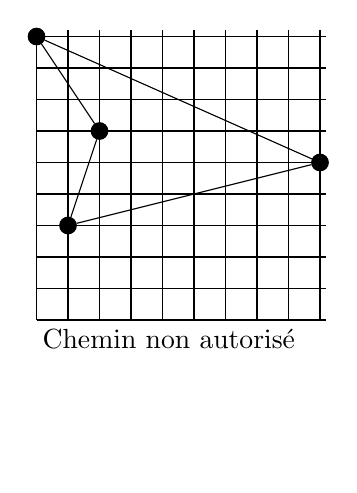
\begin{tikzpicture}[scale=.4,
    baseline={(0,0)},
    every node/.style={
        draw,
        fill=black,
        circle,
        inner sep=0pt,
        minimum size=6pt}]

    \draw (0,0) grid (9.2,9.2);

    \node (A) at (0,9) {};
    \node (B) at (1,3) {};
    \node (C) at (2,6) {};
    \node (D) at (9,5) {};

    \draw (A) -- (D) -- (B) -- (C) -- (A);

    \node[draw=none, fill=none] at (4.2, -.6) {Chemin non autorisé};
\end{tikzpicture}
\hspace{1cm}
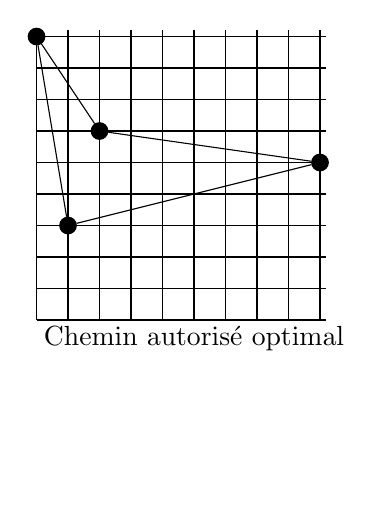
\begin{tikzpicture}[scale=.4,
    baseline={(0,0)},
    every node/.style={
        draw,
        fill=black,
        circle,
        inner sep=0pt,
        minimum size=6pt}]

    \draw (0,0) grid (9.2,9.2);

    \node (A) at (0,9) {};
    \node (B) at (1,3) {};
    \node (C) at (2,6) {};
    \node (D) at (9,5) {};

    \draw (A) -- (C) -- (D) -- (B) -- (A);

    \node[draw=none, fill=none] at (5, -.6) {Chemin autorisé optimal};
\end{tikzpicture}
\vspace{-1cm}

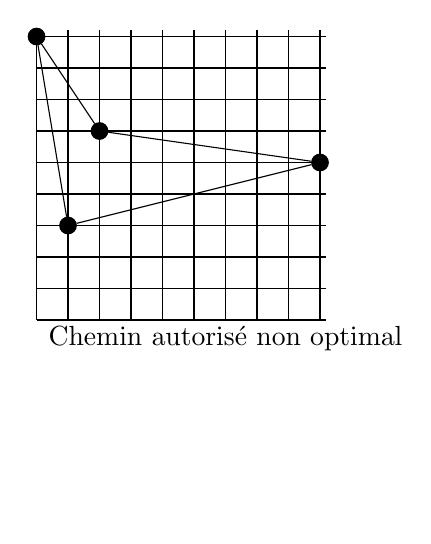
\begin{tikzpicture}[scale=.4,
    every node/.style={
        draw,
        fill=black,
        circle,
        inner sep=0pt,
        minimum size=6pt}]

    \draw (0,0) grid (9.2,9.2);

    \node (A) at (0,9) {};
    \node (B) at (1,3) {};
    \node (C) at (2,6) {};
    \node (D) at (9,5) {};

    \draw (A) -- (C) -- (D) -- (B) -- (A);

    \node[draw=none, fill=none] at (6, -.6) {Chemin autorisé non optimal};
\end{tikzpicture}
\vspace{-2cm}

\Q
Proposer un algorithme qui donne le plus court des chemins autorisés. Justifier votre algorithme. Évaluer (en fonction de $n$) un ordre de grandeur du temps qu'il nécessite, en supposant qu'une addition ou une comparaison prennent une unité de temps.

\Q
Si maintenant tous les chemins possibles sont autorisés, votre algorithme de la question précédente donne-t-il toujours un chemin de longueur minimale ?

\Corrige

\Q
Ce problème est un cas particulier du \og problème du voyageur de commerce \fg{} dans lequel on recherche un circuit optimal dit \og bitonique \fg{}. Un algorithme efficace utilise la programmation dynamique.
\medskip

On note $(p_1, p_2, ..., p_n)$ l'ensemble des points du plan correspondant aux maisons ordonnées par abscisse croissante. On appelle \og chemin bitonique \fg{} $P_{i,j}$ (où $i \leq j$), un chemin incluant les points $p_1$, $p_2$, ..., $p_j$ qui commence à un point $p_i$, va jusqu'au point $p_1$ en allant toujours dans le sens des abscisses décroissantes puis va jusqu'au point $p_j$ en allant toujours dans le sens des abscisses croissantes. Notons que $p_j$ est le point le plus à droite dans $P_{i,j}$ et fait partie du sous-chemin de $P_{i,j}$ allant vers la droite. On cherche donc ici le chemin bitonique $P_{n,n}$ de taille minimale.
\medskip

On note $|p_i, p_j|$ la distance euclidienne entre les points $p_i$ et $p_j$ et on note $b_{i,j}$ (où $i \leq j$) la longueur du chemin bitonique $P_{i,j}$ le plus court. La seule valeur $b_{i,i}$ dont nous avons besoin est $b_{n,n}$, correspondant à la longueur recherchée. On a la formule suivante pour $b_{i,j}$ avec $1 \leq i \leq j \leq n$ :
\smallskip

\hspace*{.5cm}$b_{1,2} = |p_1,p_2|$ \quad ;\\
\hspace*{.5cm}$b_{i,j} = b_{i,j-1}+|p_{j-1},p_j|$ pour $i < j-1$ \quad ;\\
\hspace*{.5cm}$b_{j-1,j} = \displaystyle\min_{1 \leq k < j-1}\,(b_{k,j-1}+|p_k,p_j|)$.

En effet, dans tout chemin bitonique se terminant par $p_2$, $p_2$ est le point d'abscisse maximale. Sa longueur est donc $|p_1,p_2|$.
\medskip

On considère maintenant le chemin bitonique $P_{i,j}$ le plus court. Le point $p_{j-1}$ se trouve quelque part sur ce chemin. S'il se trouve sur le sous-chemin allant vers la droite, alors il précède immédiatement $p_j$. Sinon, il se trouve sur le sous-chemin allant vers la gauche et il est le point le plus à droite donc $i=j-1$.\\
Dans le premier cas, le sous-chemin de $p_i$ à $p_{j-1}$ est forcément le chemin bitonique $P_{i,j-1}$ le plus court, sans quoi on pourrait le remplacer par un chemin $\tilde{P}_{i,j-1}$ plus court et on obtiendrait un chemin plus court que $P_{i,j}$ : absurde. La longueur de $P_{i,j}$ est donc donnée par $b_{i,j-1}+|p_{j-1},p_j|$.\\
Dans le second cas, $p_j$ a un prédécesseur immédiat $p_k$ (où $k<j-1$) sur le sous-chemin allant vers la droite. Par le même argument que précédemment, le sous-chemin de $p_k$ à $p_{j-1}$ est forcément $P_{k,j-1}$. La longueur de $P_{i,j}$ est donc donnée par $\displaystyle\min_{1 \leq k < j-1}\,(b_{k,j-1}+|p_k,p_j|)$.
\medskip

Dans un chemin bitonique optimal $P_{n,n}$, l'un des points adjacents à $p_n$ est nécessairement $p_{n-1}$. On a donc : $b_{n,n}=b_{n-1,n}+|p_{n-1},p_n|$.
\medskip

Pour reconstruire les points du chemin bitonique optimal $P_{n,n}$, on définit une matrice \texttt{b} de taille $(n \times n)$ pour stocker les valeurs $b_{i,i}$ et une matrice \texttt{r} telle que \texttt{r.(i-1).(j-1)} contient le prédécesseur immédiat de $p_j$ dans le chemin bitonique $P_{i,j}$ le plus court.
\medskip

L'algorithme comporte une première boucle qui itère sur tous les points puis la recherche du minimum a une complexité en $O(n)$. On a donc une complexité temporelle totale en $O(n^2)$.

\Q
L'algorithme ne donne pas la longueur minimale dans le cas général (voyageur de commerce sans la contrainte des abscisses toujours croissantes puis toujours décroissantes). Il suffit de voir les exemples de l'énoncé, où le plus court chemin autorisé est de longueur supérieure à celle du chemin non autorisé.
\bigskip

\Fin
